%%%%%%%%%%%%%%%%%%%%%%%%%%%%%%%%%%%%%%%%%
% Beamer Presentation
% LaTeX Template
% Version 1.0 (10/11/12)
%
% This template has been downloaded from:
% http://www.LaTeXTemplates.com
%
% License:
% CC BY-NC-SA 3.0 (http://creativecommons.org/licenses/by-nc-sa/3.0/)
%
%%%%%%%%%%%%%%%%%%%%%%%%%%%%%%%%%%%%%%%%%

%----------------------------------------------------------------------------------------
%	PACKAGES AND THEMES
%----------------------------------------------------------------------------------------

\documentclass{beamer}

\mode<presentation> {

% The Beamer class comes with a number of default slide themes
% which change the colors and layouts of slides. Below this is a list
% of all the themes, uncomment each in turn to see what they look like.

%\usetheme{default}
%\usetheme{AnnArbor}
%\usetheme{Antibes}
%\usetheme{Bergen}
%\usetheme{Berkeley}
%\usetheme{Berlin}
%\usetheme{Boadilla}
%\usetheme{CambridgeUS}
%\usetheme{Copenhagen}
%\usetheme{Darmstadt}
%\usetheme{Dresden}
%\usetheme{Frankfurt}
%\usetheme{Goettingen}
%\usetheme{Hannover}
%\usetheme{Ilmenau}
%\usetheme{JuanLesPins}
%\usetheme{Luebeck}
\usetheme{Madrid}
%\usetheme{Malmoe}
%\usetheme{Marburg}
%\usetheme{Montpellier}
%\usetheme{PaloAlto}
%\usetheme{Pittsburgh}
%\usetheme{Rochester}
%\usetheme{Singapore}
%\usetheme{Szeged}
%\usetheme{Warsaw}

% As well as themes, the Beamer class has a number of color themes
% for any slide theme. Uncomment each of these in turn to see how it
% changes the colors of your current slide theme.

%\usecolortheme{albatross}
\usecolortheme{beaver}
%\usecolortheme{beetle}
%\usecolortheme{crane}
%\usecolortheme{dolphin}
%\usecolortheme{dove}
%\usecolortheme{fly}
%\usecolortheme{lily}
%\usecolortheme{orchid}
%\usecolortheme{rose}
%\usecolortheme{seagull}
%\usecolortheme{seahorse}
%\usecolortheme{whale}
%\usecolortheme{wolverine}

%\setbeamertemplate{footline} % To remove the footer line in all slides uncomment this line
%\setbeamertemplate{footline}[page number] % To replace the footer line in all slides with a simple slide count uncomment this line

%\setbeamertemplate{navigation symbols}{} % To remove the navigation symbols from the bottom of all slides uncomment this line

\setbeamertemplate{frametitle}[default][center]
}

\usepackage{graphicx} % Allows including images
\usepackage{booktabs} % Allows the use of \toprule, \midrule and \bottomrule in tables
\usepackage{multimedia}
%\usepackage{movie15}
\usepackage{caption}
\usepackage{subcaption}
\usepackage{amsfonts}
\usepackage{epstopdf}
\usepackage{bigints}
\usepackage{amsmath}
\usepackage{hyperref}
\usepackage{verbatim}
\usepackage{mathrsfs}
\usepackage{color}
\usepackage[outline]{contour}
\usepackage{multirow}

\contourlength{1pt}

\newcommand\Bo{\mbox{\textit{Bo}}}  % Bond number
\newcommand\Rey{\mbox{\textit{Re}}}  % Reynolds number
\newcommand\Ri{\mbox{\textit{Ri}}}  % Richardson number

\def\Xint#1{\mathchoice
{\XXint\displaystyle\textstyle{#1}}%
{\XXint\textstyle\scriptstyle{#1}}%
{\XXint\scriptstyle\scriptscriptstyle{#1}}%
{\XXint\scriptscriptstyle\scriptscriptstyle{#1}}%
\!\int}
\def\XXint#1#2#3{{\setbox0=\hbox{$#1{#2#3}{\int}$}
\vcenter{\hbox{$#2#3$}}\kern-.5\wd0}}
\def\ddashint{\Xint=}
\def\dashint{\Xint-}

%----------------------------------------------------------------------------------------
%	TITLE PAGE
%----------------------------------------------------------------------------------------

\title[Modeling volcanic processes]{Magma generation and properties} % The short title appears at the bottom of every slide, the full title is only on the title page

\author[Paul Jarvis]{Paul A. Jarvis} % Your name
\institute[UNIGE] % Your institution as it will appear on the bottom of every slide, may be shorthand to save space
{
\textit{paul.jarvis@unige.ch} % Your email address
}
\date{15th November 2019} % Date, can be changed to a custom date
\begin{columns}

  \begin{column}{0.33\paperwidth}
    $$\includegraphics[width=0.3\paperwidth]{UNIGE_logo.jpg}$$
  \end{column}

  \begin{column}{0.33\paperwidth}
    $$\includegraphics[width=0.3\paperwidth]{redoubt.jpg}$$
  \end{column}

  \begin{column}{0.33\paperwidth}
    $$\includegraphics[width=0.3\paperwidth]{etna.jpg}$$
  \end{column}
  
\end{columns}
\vspace{-2cm}

\DeclareMathOperator\erf{erf}

\begin{document}

\begin{frame}
\titlepage % Print the title page as the first slide
\end{frame}

%\begin{frame}
%\frametitle{Overview} % Table of contents slide, comment this block out to remove it
%\tableofcontents % Throughout your presentation, if you choose to use \section{} and \subsection{} commands, these will automatically be printed on this slide as an overview of your presentation
%\end{frame}


%----------------------------------------------------------------------------------------
%	PRESENTATION SLIDES
%----------------------------------------------------------------------------------------

%------------------------------------------------
%\section{First Section} % Sections can be created in order to organize your presentation into discrete blocks, all sections and subsections are automatically printed in the table of contents as an overview of the talk
%------------------------------------------------

%\subsection{Subsection Example} % A subsection can be created just before a set of slides with a common theme to further break down your presentation into chunks

\begin{frame}
  \frametitle{What is magma?}

  \begin{itemize}
  \item Naturally occurring \textbf{molten} or partially molten rock material, generated within the Earth and capable of \textbf{intrusion} and \textbf{extrusion}, from which igneous rocks are derived through \textbf{solidification} and related processes. It may or may not contain \textbf{suspended solids} (such as crystals and rock fragments) and/or \textbf{gas phases}.
  \end{itemize}

  \hfill (Glossary of Geology, 2011)

  \begin{columns}

    \begin{column}{0.45\paperwidth}

      \vspace{-1cm}

      Magma is
      \begin{itemize}
      \item \textbf{three-phase}:
        
        \begin{itemize}
        \item \textbf{solid} - unmelted crystals \\
        \item \textbf{liquid} - molten rock      \\
        \item \textbf{gas} - exsolved volatiles  \\
        \end{itemize}
        
      \item \textbf{multi-component}:
        
        \begin{itemize}
        \item Many chemical species \\
        \item SiO$_{2}$, K$_{2}$O, Na$_{2}$O, H$_{2}$O, etc.
        \end{itemize}
        
      \end{itemize}

    \end{column}

    \begin{column}{0.45\paperwidth}
      $$\includegraphics[width=0.45\paperwidth]{3_phase.png}$$

    \end{column}
    
  \end{columns}
  
\end{frame}
%-----------------------------------------------

\begin{frame}
  \frametitle{Thermodynamic controls on magma properties}

  Physical and chemical properites of magma are controlled by three parameters:

  \begin{itemize}
  \item Temperature $T$ \\
  \item Pressure $P$ \\
  \item Bulk composition $\mathbf{X} = (X_{\text{SiO}_{2}}, X_{\text{K}_{2}\text{O}}, X_{\text{Na}_{2}\text{O}}, X_{\text{H}_{2}\text{O}}, \text{...})$ \\
  \end{itemize}

  $$ \sum_{i} X_{i} = X_{\text{SiO}_{2}} + X_{\text{K}_{2}\text{O}} + X_{\text{Na}_{2}\text{O}} + X_{\text{H}_{2}\text{O}} + ... = 1 $$
  
  $X_{i} =$ Fraction of the i$^{\text{th}}$ component ($i = $ SiO$_{2}$, K$_{2}$O, Na$_{2}$O, H$_{2}$O, ...)
  
\end{frame}
%-----------------------------------------------

\begin{frame}
  \frametitle{Magma composition: Dry classification}

  Classification normally performed according to a subset of components \\

  \vspace{0.5cm}

  Volcanic rocks often classified on a \textbf{Total Alkali Silica (TAS)} diagram \\

  \begin{columns}[t]

    \begin{column}{0.45\paperwidth}

      \vspace{-0.8cm}
      
      $$\includegraphics[width=\textwidth]{TAS.JPG}$$
      
    \end{column}

    \begin{column}{0.45\paperwidth}

      SiO$_{2}$ normally largest component ($\sim$ 37-77) wt\% \\

      \vspace{0.5cm}

      $X_{\text{SiO}_{2}}, X_{\text{K}_{2}\text{O}}, X_{\text{Na}_{2}\text{O}}$ determine composition of many crystals \\

      \vspace{0.5cm}

      Not suitable for all volcanic rocks e.g. High MgO \\
    \end{column}
  \end{columns}

  \vspace{0.5cm}
  
  Le Maitre et al. (2002) Igneous Rock: A Classification and Glossary of Terms \\
\end{frame}
%-----------------------------------------------

\begin{frame}
  \frametitle{Magma composition: volatile content}

  Magmas can contain dissolved gas species \\

  \vspace{0.5cm}

  H2O and CO2 are most abundant, then S, Cl and F \\

  \vspace{0.5cm}

  \textbf{Solubility} - Maximum amount of a species that can be dissolved \\
  \hspace{1.5cm} - depends on $P, T, \mathbf{X}$ \\

  \vspace{0.5cm}

  Once solubility exceeded, bubbles of exsolved phases form (\textbf{vesiculation})\\

  \vspace{0.5cm}

  Consequnces for:

  \begin{columns}[t]
    \begin{column}{0.33\paperwidth}
        \begin{itemize}
        \item Crystallisation
        \item Density
        \item Viscosity
        \end{itemize}
    \end{column}

    \begin{column}{0.33\paperwidth}
      \vspace{-1cm}
      
      $$\includegraphics[width=\textwidth]{arrow.png}$$
    \end{column}

    \begin{column}{0.33\paperwidth}
      \vspace{0.2cm}
      
        \begin{itemize}
        \item Eruptability
        \item Eruptive style
        \end{itemize}
    \end{column}

  \end{columns}
  \end{frame}
%-----------------------------------------------

\begin{frame}
  \frametitle{Magma generation - How to melt rocks?}

  \begin{columns}[t]
    \begin{column}{0.5\paperwidth}
      $$\includegraphics[width=0.95\textwidth]{geotherm.png}$$
    \end{column}

    \begin{column}{0.5\paperwidth}
      $$\includegraphics[width=0.95\textwidth]{Earth_crop.png}$$
    \end{column}

  \end{columns}
  
  \end{frame}
%-----------------------------------------------

\begin{frame}
  \frametitle{Magma generation - How to melt rocks?}

  \vspace{-0.5 cm}
  
  \begin{columns}[t]
    \begin{column}{0.5\paperwidth}
      $$\includegraphics[width=0.95\textwidth]{heating.png}$$
    \end{column}

    \begin{column}{0.5\paperwidth}

      \begin{itemize}
      \item \textbf{Heating}: Increase $T$ \\
        \begin{itemize}
          \item Hot spot volcanism
        \end{itemize}
      \end{itemize}

      \vspace{-0.8cm}
      
      $$\includegraphics[width=0.95\textwidth]{plume_melting.png}$$

    \end{column}

  \end{columns}
  
  \end{frame}
%-----------------------------------------------

\begin{frame}
  \frametitle{Magma generation - How to melt rocks?}

  \vspace{-0.5 cm}
  
  \begin{columns}[t]
    \begin{column}{0.5\paperwidth}
      $$\includegraphics[width=0.95\textwidth]{depressure.png}$$

      \vspace{-0.6cm}

      $$ \left.\frac{\mathrm{d} T}{\mathrm{d} P}\right|_{\Delta S = 0} = \frac{\alpha T}{\rho C_{p}}$$
      
    \end{column}

    \begin{column}{0.5\paperwidth}

      \begin{itemize}
      \item \textbf{Depressurisation}: Reduce $P$ \\
        \begin{itemize}
          \item Mid-ocean ridge volcanism
        \end{itemize}
      \end{itemize}

      $$\includegraphics[width=0.95\textwidth]{decompression_melting.png}$$

      $\alpha =$ Thermal expansion coefficient \\
      $\rho = $ Density \\
      $C_{p}$ = Heat capacity \\
      $\Delta S = $ Change in entropy \\
    \end{column}

  \end{columns}
  
  \end{frame}
%-----------------------------------------------

\begin{frame}
  \frametitle{Magma generation - How to melt rocks?}

  \begin{columns}[t]
    \begin{column}{0.5\paperwidth}
      $$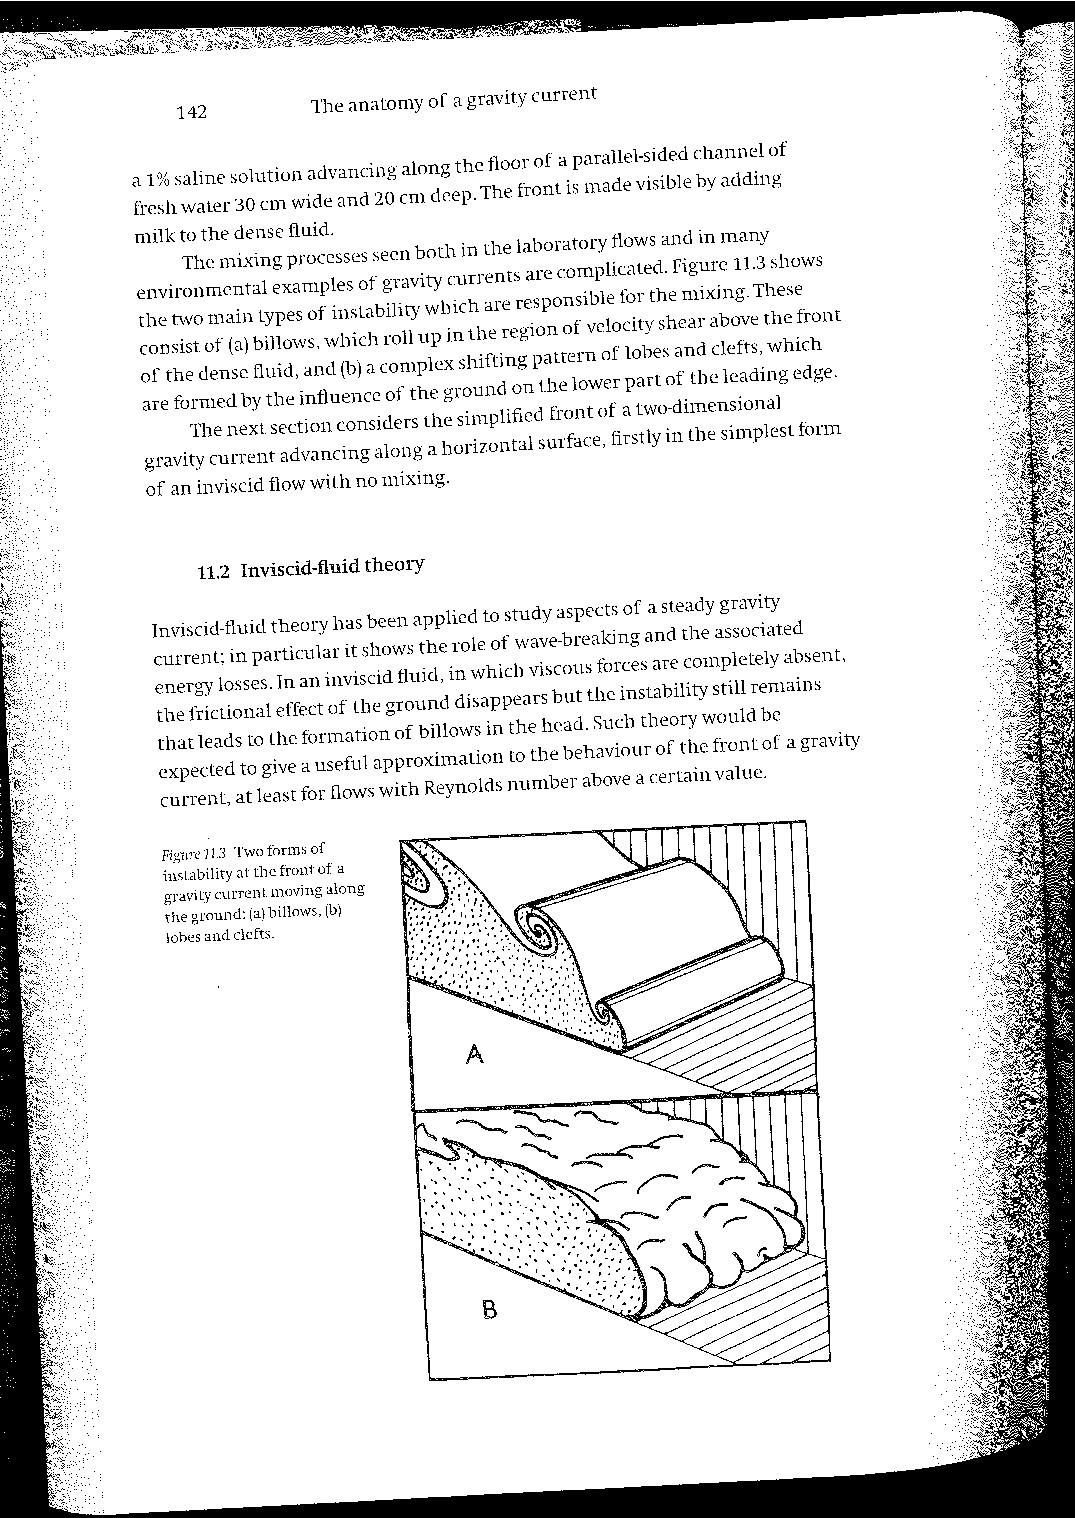
\includegraphics[width=0.95\textwidth]{mixing.png}$$
    \end{column}

    \begin{column}{0.5\paperwidth}

      \begin{itemize}
      \item \textbf{Compositional change}: Change $\mathbf{X}$ \\
        \begin{itemize}
          \item Arc volcanism
        \end{itemize}
      \end{itemize}

      $$\includegraphics[width=0.95\textwidth]{flux_melting.png}$$

      \small Decreasing $X_{\text{H}_{2}\text{O}}$ shifts solidus to smaller $T$
      
    \end{column}

  \end{columns}
  
  \end{frame}
%-----------------------------------------------

\begin{frame}
  \frametitle{Phase diagrams}

  \vspace{-0.5cm}
  
  \begin{columns}[t]
    \begin{column}{0.45\paperwidth}
      $$\includegraphics[width=\textwidth]{plag_phase.png}$$

      Three parameters can be considered on a ternary phase diagram \\

      \vspace{0.5cm}
      
      All diagrams are just \textit{slices} of the full picture \\
    \end{column}

    \begin{column}{0.5\paperwidth}

      State of magma depends on many parameters ($T, P, X_{i}$) \\

      Can consider two parameters on a simple \textbf{binary} phase diagram\\

      Determine compositions and relative proportions of different phases \\

      \vspace{-0.8cm}

      $$\includegraphics[width=0.95\textwidth]{ternary.png}$$
      
    \end{column}

  \end{columns}
  
  \end{frame}
%-----------------------------------------------


\end{document}
